\chapter{基于一致性预测的无人机集群分类不确定量化研究}
\label{chap:Swarm-MCP}

\section{引言}
以实际工程任务中无人机集群行为分类的不确定量化设计问题为背景, 本章重点研究基于Boosting底层机器学习算法, 为无人机集群行为分类研究提供不确定量化求解。

现有关于无人机集群行为分类的研究大都集中于如何利用机器学习算法给出分类结果, 这种模式下得到的结果通常是简单预测, 无法针对具体的预测结果提供置信程度的评价。尽管它们在总体上都能够保证取得不错的分类效果, 但是在针对具体预测输出结果上仍然无法提供具有针对性的不确定量化。因此, 针对这类复杂无人机集群行为分类问题, 本章基于一致性预测算法的思想, 提出采用蒙德里安一致性预测(Mondrian Conformal Prediction, MCP)框架为利用各种机器学习算法求解无人机集群行为分类提供精确有效的不确定量化研究。

从理论来看, 第\ref{chap:edbed}章关于机器学习理论的介绍已经表明基于强收敛模式下一致收敛的统计学习理论给出的结论是断言, 这种学习模型属于现象学学习模型\citep{vapnik2020,Husserl1937,wangdefeng-xianxiangxue-2005}。 通过现象学学习理论可知机器学习算法的输出是一个暴力得分\citep{vapniktalk2015}, 其取值缺乏置信程度的度量, 仅仅可根据机器学习输出结果得到分类标识而不能据此展开任何不确定程度的度量\citep{2006Hedging}。

正因为如此, 众多学者提出多种校正方法以期为暴力得分赋予概率意义上的取值。 这些校正方法中最有名的是Platt校正方法, 这种校正方法也是目前各种开源软件包中默认采用的方法\citep{Platt1999}。 但是仔细看来——正如Vapnik所言——Platt校正方法把SVMs退化为模型驱动方法\citep{Vapnik2021}。本来借助Vapnik提出的SVMs方法, 经验数据获得其超越表征(这是真正意义上的数据驱动), 然而Platt通过假设这些输出函数服从Sigmoid函数而将原本纯粹数据驱动算法转变为模型驱动算法\citep{Vapnik-Synergy-2016}。

一致性预测也是通过为机器学习算法的输出提供有效校正的角度出发的。一致性预测考虑给出的是集合预测, 即预测算法要求输出第$n$个观测所有可能的结果。区别于传统统计学中区间估计失效的现实\citep{Herbert1995,Herbert1998,Herbert2001,Ioannidis2005,Taylor2015,Tibshirani2015,Wasserstein2016,Altman2017,Andrade2019,Betensky2019,Lee2019,Ioannidis2019}, 一致性预测总能给出自动有效的区间估计。即当给定显著性水平$\epsilon$, 一致性预测出错的频率是严格受到控制的, 并且如果随机性假设被满足——比如采用技术手段随机化样本数据——那么犯错的频率是被精确控制的。 一致性预测算法得到的有效误差控制是无需任何分布假设的(因为根据第二章的理论可知, 底层现代机器学习算法(以SVMs为例)无需分布假设\citep{Cortes1995}), 是一种无分布假设的不确定量化算法框架。


\section{一致性预测理论研究}
本节首先针对一致性预测算法给出理论介绍, 然后再针对无人机集群行为预测的不确定量化给出具体的算法建模。

考虑机器学习中的分类问题, 基于观测样本空间, 目的为新观测对象$x_{n}$预测其真实标签$y_{n}$。 对于任意样本序列$(x_{1}, y_{1}), \ldots, (x_{n-1}, y_{n-1}) \in \mathbf{Z}^{*}$ 以及任意的新对象$x_{n} \in \mathbf{X}$, 机器学习算法给出的结果可以表述为下列映射关系:
\begin{align}
\label{simple-prediction}
D: \mathbf{Z}^{*} \times \mathbf{X} \rightarrow \mathbf{Y}.
\end{align}
将这样的机器学习算法称作简单预测。 此函数根据机器给出的新对象$x_{n}$的暴力得分函数得到预测标签$y_{n}$。

现在需要为此暴力标签给出置信预测, 即为暴力标签补充提供到底其可信程度是多少, 然后再尝试提供一个在指定显著水平下的集合预测。因为对于复杂问题, 一旦单值预测出错, 那么提供的集合预测则可以对单值出错情形给出有效的校正。

一致性预测基于提前给定的显著性水平$\epsilon \in (0, 1)$, 新对象的集合预测$\Gamma$可以表述为下列形式:
\begin{align}
\label{confidence-predictor}
\Gamma: \mathbf{Z}^{*} \times \mathbf{X} \times (0, 1) \rightarrow 2^{\mathbf{Y}}
\end{align}
其中, 这里$2^{\mathbf{Y}}$是类别集合$\mathbf{Y}$的势。

集合预测$\Gamma$的输出结果
\begin{align}
\label{confidence-output}
\Gamma^{\epsilon}(x_{1}, y_{1}, \ldots, x_{n-1}, y_{n-1}, x_{n})
\end{align}
必须满足下列关系式
\begin{align}
\Gamma^{\epsilon_{1}}(x_{1}, y_{1}, \ldots, x_{n-1}, y_{n-1}, x_{n}) \subseteq \Gamma^{\epsilon_{2}}(x_{1}, y_{1}, \ldots, x_{n-1}, y_{n-1}, x_{n})
\end{align}
其中这里的$\epsilon_{1} \geq \epsilon_{2}$。 在置信水平$1 - \epsilon$下, 集合预测$\Gamma$宣布新对象的标签$y_{n}$在其预测集合中, 即
\begin{align}
\label{confidence-y}
y_{n} \in \Gamma^{\epsilon}(x_{1}, y_{1}, \ldots, x_{n-1}, y_{n-1}, x_{n}).
\end{align}

如果集合预测$\Gamma$的预测集合不包含任何标签, 称之为空元素集合预测; 如果集合预测$\Gamma$的预测集合只包含一个标签(并不需要必须要求此标签就是真实标签)就称之为单元素集合预测; 如果集合预测$\Gamma$的预测集合包含多个标签, 称之为多元素集合预测。 如果真实标签$y_{n}$不被以上三种预测结果所包含, 那么就称集合预测$\Gamma$输出错误预测。 因此, 这样说来对于多元素集合预测, 如果输出结果为多元素但是包含真实标签, 并不视这种情形为预测错误, 这仅仅表明集合预测$\Gamma$并没有提供高效的信息而已。显然, 预测集合在尽可能包含真实标签的同时集合元素的个数越少越好, 这就意味着置信预测给出的结果是高效的。

根据一致性预测计算得到p-值后, 就会很容易获得置信预测。置信预测具有两个显著的特征: 置信度和可信度。其中置信度表征预测的有效性(validity), 可信度表征预测的高效性(efficiency)。 给定显著性水平 $\epsilon$, 如果预测错误的相对频率在任意给定的显著性水平$\epsilon$下不超过$\epsilon$, 这样的预测是有效的。 这就意味着在用户指定的任意显著性水平下机器都能够给出有效的预测结果, 而对于可信度则意味着预测结果能给出更多信息。 

针对具体的机器学习算法而言, 一致性预测的确能够为任意的机器学习算法提供可信的不确定性度量。这是因为一致性预测方法是以机器学习算法的输出作为开端的。 因此, 一致性预测方法也被视作是可信机器学习算法的一种完整的实现。 

在继续阐述一致性预测之前, 需要引进一个新的概念: “袋子”。 “袋子”也称作是“多元素集合”, 即在“袋子”中的元素是忽略顺序——这一点与“集合”是相同的; 与此同时“袋子”允许出现完全一样的元素——这一点与“集合”不一样。 容量为$n$的“袋子”指的是“袋子”中的元素的个数为$n$, 并记做 $\Lbag z_1, \ldots, z_{n} \Rbag$。 记$\mathbf{Z}^{(n)}$为来自可测空间$\mathbf{Z}$中的$n$个元素组成的大小为$n$的所有“袋子”的集合。 记 $\mathbf{Z}^{*}$是可测空间$\mathbf{Z}$的所有元素的所有“袋子”的集合。 这样一来, 一致性预测需要基于某非一致度量函数(nonconformity measure)来量测新数据$(x_{n}, y)$与已知样本序列$\Lbag z_1, \ldots, z_{n-1} \Rbag$的符合程度。 需要将待估标签的所有可能都按照这种方式计算, 进而得到每个候选标签对应的非一致性得分(nonconformity score)。 通过对非一致得分的标准化就得到每个候选标签对应的p-值。

非一致性测度的根基来源于SVMs中拉格朗日乘子$\alpha_{i}$\citep{Vovk2013,vovk2005algorithmic,vovk2022algorithmic}。 从现象学角度阐述SVMs可知拉格朗日乘子$\alpha_{i}$表征的是样本的异化程度:
\begin{enumerate}
\item 如果样本$z_{i}$对应的$\alpha_{i} = 0$, 那么表明样本$z_{i}$的异化程度最低, 这样的样本就都是经典的、平凡的;
\item 如果样本$z_{i}$对应的$\alpha_{i} = C$(这里的$C$是$\alpha$的最大取值), 那么表明样本$z_{i}$的异化程度最高, 这样的样本就是最极端、最野样本;
\item 如果样本$z_{i}$对应的$0 < \alpha_{i} < C$, 那么表明样本$z_{i}$的异化程度就介于平凡和极端之间。
\end{enumerate}

面对越极端的样本, 越有信息给出其类别标签。 因此, 非一致性测度就是评估新样本与旧样本异化程度的方法, 或者评估新样本与旧样本“有多么奇怪”。非一致性测度将每个可能的新样本和“袋子”中旧样本映射为一个数值得分, 即非一致性得分:
\begin{align}
\label{nonconformity-score}
A: \mathbf{Z}^{*} \times \mathbf{Z} \rightarrow \mathbf{R}.
\end{align}
对样本中的每个样例都执行非一致性测度, 就可以得到对于每个样本$n = 1, 2, \ldots$定义的诸非一致性测度$A_{n}$的集合
\begin{align}
\label{nonconformity-set}
A_{n}: \mathbf{Z}^{n-1} \times \mathbf{Z} \rightarrow \mathbf{R},
\end{align}
其中这里$n$是“袋子”的大小。 因此, 对于“袋子”$\Lbag z_1, \ldots, z_{n} \Rbag$中的每个样本$z_{i}$其非一致性得分定义为
\begin{align}
\label{nonconformity-score-zi}
\alpha_{i} := A_{n}(\Lbag z_1, \ldots, z_{i-1}, z_{i+1}, \ldots, z_{n} \Rbag, z_{i}).
\end{align}

非一致性得分$\alpha_{i}$自身并不能给出任何关于样本$z_{i}$与其他样本相比较的异化信息, 为此需要将这些非一致性得分纳入同一个系统以实现彼此之间的比较。 也就是说, 需要通过计算每个样本对应的p-值来指示非一致性得分$\alpha_{i}$与其他样本相比较的奇异程度。 对于样本$z_{i}$其p-值定义如下
\begin{align}
\label{p-value}
p := \frac{|\{j = 1, \ldots, n: \alpha_{j} \geq \alpha_{i}\}|}{n}.
\end{align}

p-值量化的是样本$z_{i}$与其他样本彼此之间的奇异程度。 因为在计算p-值时是利用$\alpha_{i}$彼此之间比较得到的, 因此p-值的取值范围是$[\frac{1}{n}, 1]$。 如果样本$z_{i}$的p-值非常小(计算p-值的分子是数数大于$\alpha_{i}$的个数。 p-值非常小, 即大于$\alpha_{i}$的样本少, $\alpha_{i}$本身取值很大), 这就表明样本$z_{i}$与其他样本之间是非常不一致, 亦即非常奇怪的, 异化程度是非常高的; 如果$z_{i}$的p-值非常大(计算p-值的分子是数数奇异的个数, p-值非常大, 即大于$\alpha_{i}$的样本多, $\alpha_{i}$本身取值很小), 那么就表明样本$z_{i}$与其他样本之间是非常一致的, 亦即非常相似的。 将1减去第二大p-值定义为预测的置信度, 即刻画有效性; 将最大p-值——此标签下的样本与原样本非常一致——对应的标签视为是预测的标签并且将此p-值视为可信度(即传递给的信息最丰富)。 形式化而言 \citep{2006Hedging}, 即:
\begin{align}
\textsf{置信度:} \quad &\sup\{1-\epsilon: |\Gamma^{\epsilon} \leq 1|\}, \\
\textsf{可信度:} \quad &\inf\{\epsilon: |\Gamma^{\epsilon}| = 0\}.
\end{align}
而对于置信预测算子, 则很容易得到其集合预测
\begin{align}
\Gamma^{\epsilon}(x_{1}, y_{1}, \ldots, x_{n-1}, y_{n-1}, x_{n}) := \{y \in \mathbf{Y}: p_{y} > \epsilon\}.
\end{align}
其中, 这里的$p_{y}$是数据对$(x_{n}, y)$对应的p-值, 
\begin{align}
\label{definition-of-py}
p_{y} := \frac{|i = 1, \ldots, n: \alpha_{i} \geq \alpha_{n}|}{n}.
\end{align}
其中,
\begin{align}
\alpha_{i} &= A_{n}(\Lbag (x_{1}, y_{1}), \ldots, (x_{i-1}, y_{i-1}), (x_{i+1}, y_{i+1}), \ldots, (x_{n}, y) \Rbag, (x_{i}, y_{i})),\\
\alpha_{n} &= A_{n}(\Lbag (x_{1}, y_{1}), \ldots, (x_{n-1}, y_{n-1}) \Rbag, (x_{n}, y)).
\end{align}
这样(如果在满足随机性假设条件下)就可以在任意指定置信水平$1 - \epsilon$下保证新对象$x_{n}$的真实标签$y_{n}$一定包含在预测集合$\Gamma^{\epsilon}$中。


\section{蒙德里安一致性预测不确定量化方法研究}
\label{sec:method}
本节介绍提出的蒙德里安一致性预测研究, 并将之应用于无人机集群行为分类的不确定量化研究。

首先介绍作为底层超越算子的Boosting算法。 Boosting算法的基本假设是通过一些弱学习器为给定标签的训练样本生成一个弱分类规则函数 \citep{Boosting2012}。 这里的“弱分类器”指的是优于随机猜测的分类器。 然后通过综合多个弱分类器, 进而使得整个算法的分类能力得以增强。形式化而言, Boosting算法考虑将诸训练样本
\begin{align}
(x_{1}, y_{1}), \ldots, (x_{l}, y_{l}),
\end{align}
作为算法输入, 寻找下列形式的弱分类器
\begin{align}
f(x, \alpha) : X \times Y \rightarrow [0, 1],
\end{align}
去逼近数据的分布$D_{t}$. 弱分类器的学习品质通过下列表达式测量, 即
\begin{align}
\epsilon_{t} \doteq \mathbf{Pr}_{i \sim D_{t}}[f(x_{i},\alpha_{t}) \neq y_{i}],
\end{align}
其中, 这里$\mathbf{Pr}_{i \sim D_{t}}[\cdot]$ 表示样本被随机选中的概率。 一旦得到这样的弱分类器$f(x, \alpha_{t})$, Boosting就保留其参数$\alpha_{t}$, 直观地说, 这样的参数就可视为是弱分类器重要程度的度量, 然后更新数据分布$D_{t}$。 经过若干次迭代, Boosting就可获得若干组分类效果较佳的弱分类器, 最后通过将这些弱分类器组合起来用于逼近待估函数$f(x,\alpha_{0})$ 的近似分类器$f(x, \alpha_{\text{emp}})$。

基于底层Boosting算法考虑为Boosting输出结果提供可信机器学习度量。 也就是说, 给定训练样例预测新对象的标签, 并且为预测结果给出其不确定性量化。 因此考虑输出集合预测模式。 集合预测将经验数据映射至指定显著性水平$\epsilon$下对应的集合输出$\Gamma^{\epsilon}$。 显著性水平$\epsilon \in [0,1]$反映的是针对预测结果可信程度的需求。

一致性预测(又名超越置信机(TCM)\citep{Vovk-Mondrian-2003})其原初的思想是针对超越推理(Transductive Inference)而开发的, TCM的主要缺点是计算效率低(因为按照理论要求, 针对每个样本都需要重新训练一次底层算法)\citep{2006Hedging}。 针对计算效率低的缺点, Vovk团队提出归纳范式下的一致性预测(Inductive Conformal Prediction, ICP)\citep{Papadopoulos2007}以缓解计算效率低的问题。 当然, 任何算法的改进都不是万能的, 势必带来新的问题。 ICP的主要问题是对训练数据的浪费, 因为校验数据不能参与模型的训练。 鉴于此, 提出蒙德里安一致性预测(Mondrian Conformal Prediction, MCP)来改进ICP和CP遇到的问题 \citep{vovk2005algorithmic}。 下面介绍MCP算法的基本情况. 

对于诸现实样例(reality examples)
\begin{align}
z_{1}, z_{2}, \ldots,
\end{align}
其中, 每个样例$z_{i} = (x_{i}, y_{i})$由对象$x_{i}$(即特征向量)和标签$y_{i}$组成。 这些对象组成可测空间$\mathbf{X}$——称之为对象空间——的各个元素, 这些标签是可测空间$\mathbf{Y}$——称之为对象空间——的各个元素。将训练集合$Z_{\text{training}} = (z_{1},\ldots,z_{l})$划分为两部分: 其中一部分是样本容量为$m < l$的真实训练集$Z_{\text{proper}} = (z_{1},\ldots,z_{m})$, 另一部分是样本容量为$l-m$的校验集$Z_{\text{calibration}} = (z_{m+1},\ldots,z_{l})$ \citep{shafer08a}。 中选择下列表达式作为MCP方法的非一致得分测度函数, 
\begin{align}
K : Z^{m} \times Z \rightarrow \mathbf{K},
\end{align}
其中, 这里$\mathbf{K}$ 是一个可测空间, 对应于$K$的非一致得分定义为下列表达式, 
\begin{align}
\alpha_{i} &:= A((z_{1}, \ldots, z_{m}), z_{i}), i = m+1, \ldots, l,\\
\alpha^{y} &:= A((z_{1}, \ldots, z_{m}), (x, y)),
\end{align}
并且对应的p-值被定义为下列形式,
\begin{align}
\label{p-value}
p^{y} := \frac{|\{i = m + 1, \ldots, l | k_{i} = k^{y},  \alpha_{i} \leq \alpha^{y}\}| + 1}{|\{i = m + 1, \ldots, l | k_{i} = k^{y}\}| + 1}.
\end{align}
采用下列函数来度量非一致性测度
\begin{align}
\label{margin}
\alpha_{i} = 0.5 - \frac{\hat{v}(y_{i} | x_{i}) - \max_{y \in \mathbf{Y} \wedge y \neq y_{i}}^{}\hat{v}(y|x_{i})}{2}.
\end{align}
其中, 这里的$\hat{v}(\cdot)$是关于$x_{i}$的样本底层机器学习算法输出的暴力预测得分。 使用MCP来校正这一得分并且计算有效的p-值, 通过计算得到的p-值序列可以据此构建集合预测并且给出相应置信度和可信度。 

输出两种模式的预测结果, 置信预测和集合预测。 对于置信预测MCP方法会将p-值最大的标签作为此样本的预测标签, 即
\begin{align}
\Gamma_{\text{simple}} = \{c | \max (p^{y})\}.
\end{align}
同时, 两个重要的不确定性量度指标——置信度和可信度——也可以通过下列定义取得\citep{2006Hedging}, 即:
\begin{align}
\label{confidence-credibility}
\textsf{置信度:} \quad &\sup\{1-\epsilon: |\Gamma^{\epsilon} \leq 1|\}, \\
\textsf{可信度:} \quad &\inf\{\epsilon: |\Gamma^{\epsilon}| = 0\},
\end{align}
这里, 与先前一样选择最大的p-值作为可信度, 1减去第二大p-值作为置信度。显著性水平$\epsilon \in (0,1)$由用户确立。 而对于MCP方法的集合预测$\Gamma^{\epsilon} = \{y \in \mathbf{Y}: p^{y} > \epsilon\}$, MCP方法能够确保在置信水平$1-\epsilon$下, 所得的集合预测是能够确保其一定包含真实标签的。 按照这种方法, 可以得到在任意指定显著性水平$\epsilon$下, MCP方法总是能够给出有效的集合预测。 有关基于Boosting算法的MCP方法的细节, 将在算法\ref{alg:mcp}中呈现, 此算法详细给出简单预测和集合预测两种预测结果。
\begin{algorithm}[]
    \small
    \caption{MCP-Boosting 算法}\label{alg:mcp}
    \hspace*{\algorithmicindent} \textbf{输入:} {$Z_{\text{proper}}$, $Z_{\text{calibration}}$, $\mathbf{X}_{\text{test}}$, $\epsilon$.}\\
    \hspace*{\algorithmicindent} \textbf{输出:} {置信预测结果或者集合预测结果.}
    \begin{algorithmic}[1]
        \Procedure{MCP-Boosting}{}
        \State {使用数据集$Z_{\text{proper}}$训练Boosting算法$T$,}
        \For{$z_{m+i} \in Z_{\text{calibration}}$}
        \For{$y \in \mathbf{Y}$}
        \State  使用表达式(\ref{margin})计算 $\alpha_{m+i}$,
        \EndFor
        \EndFor
        \For{$z_{l+i} \in$ $Z_{\text{test}}$}
        \For{$y \in \mathbf{Y}$}
        \For{$(x_{l+i},y)$}
        \State  使用表达式(\ref{margin}) 计算 $\alpha_{l+i}^{y}$,
        \State  使用表达式(\ref{p-value}) 计算 $p_{l+i}^{y}$,
        \State 根据表达式(\ref{confidence-credibility})计算置信度和可信度,
        \EndFor
        \EndFor
        \EndFor
        \While{置信预测}
        \State 计算置信预测标签: $\Gamma_{\text{simple}} = \{y: \max(p_{}^{y})\}$,
        \State 计算置信度: $\sup\{1-\epsilon: |\Gamma^{\epsilon} \leq 1|\}$,
        \State 计算可信度: $\inf\{\epsilon: |\Gamma^{\epsilon}| = 0\}$,
        \EndWhile
        \While{集合预测}
        \State 计算集合预测结果: $\Gamma_{}^{\epsilon} = \{y: p_{}^{y} > \epsilon\}$.
        \EndWhile
        \EndProcedure
    \end{algorithmic}
\end{algorithm}



\section{基于蒙德里安一致性预测的无人机集群分类}
\label{sec:results} 

根据以上关于一致性预测的理论介绍, 本节为无人机集群行为分类展开不确定量化研究。无人机集群行为分类一致性预测研究方案设计框架如图\ref{fig:MCP-framework}所示, 即基于任意底层机器学习算法, 利用蒙德里安一致性预测(Mondrian Conformal Prediction, MCP)理论为机器学习算法的输出结果提供置信预测和集合预测两种模式的不确定量化。

\begin{figure}[]
\centering
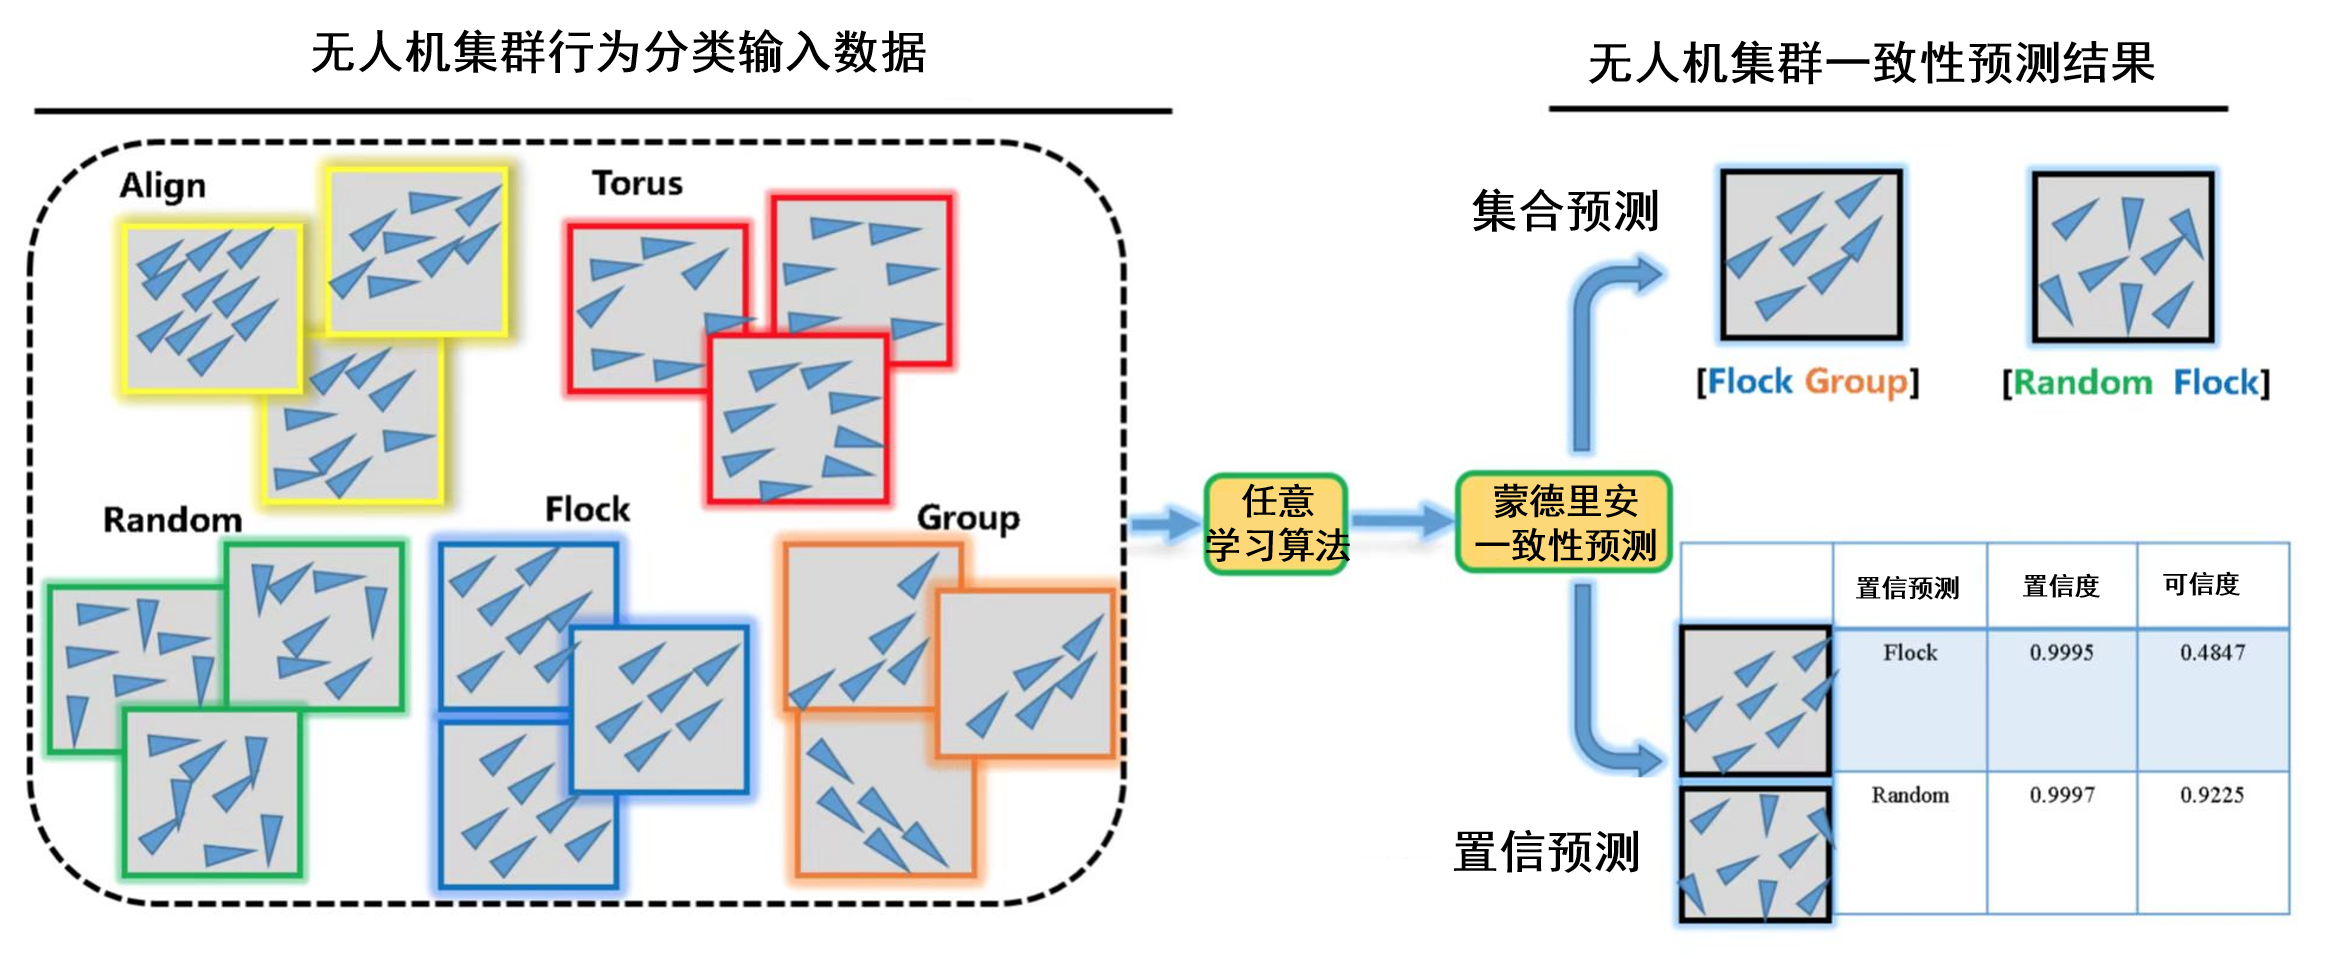
\includegraphics[width=1\linewidth]{Img/chapter8/MCP}
\caption{无人机集群行为分类蒙德里安一致性预测方案框架图}
\label{fig:MCP-framework}
\end{figure}

首先介绍获取无人机集群数据建模, 分别介绍两种集群行为数据集, 即仿真无人机集群数据集(多类别分类问题)和真实无人机集群行为数据集(二元分类问题)。

\subsection{仿真无人机集群行为数据}
\label{sec:dynamic}
对于无人机集群行为的仿真数据, 动力学模型来自于\citet{Flocks1987}。 按照\citet{Thomas2021}给出的\citet{Flocks1987}动力学模型, 有
\begin{align}
F_{ri} &= \sum_{j=1}^{N_{r}}\frac{x_{i} - x_{j}}{||x_{i} - x_{j}||^{2}},\\
F_{ai} &= \sum_{j=1}^{N_{a}}v_{j} - v_{i},\\
F_{hi} &= x_{h_{i}} - x_{i},\\
F_{fi} &= -v_{i}\frac{(||v_{i}|| - s)}{s}.
\end{align}
其中, 这里$N_{r}, N_{a}$分别表示位于排斥力(repulsion)和对齐力(alignment)域内的智能体的数量, $x_{h}$表示中心位置(home location), $r_r$ 和 $r_a$ 分别表示排斥力和对齐力的作用半径, $||\cdot||$ 表示欧式范数。 $x_{i}$ 和 $v_{i}$ 表示位置信息和速度信息。 因此, 动力学模型中智能体所受的合力可表述为下列表达式:
\begin{align}
F_{i}(t) = K_{a}F_{ai} + K_{r}F_{ri} + K_{f}F_{fi} + K_{h}F_{hi},
\end{align}  
其中, 这里的系数$K$确定智能体所受各种力的比例属性。 在动力学模型中, 还为受力模型加入一层非线性过滤函数, 即对于终端的输出, 按照下列表达式
\begin{align}
F_{i}(t) \mapsto \alpha \tanh (\beta F_{i}(t)),
\end{align}
其中, 这里设置不同的$\alpha$和$\beta$系数以产生不同的集群行为。

对于每个智能体, 假设固定的单位质量, 那么系统的更新按照如下表达式完成:
\begin{align}
\ddot{x}_{i}(t) = F_{i}(t).
\end{align}
对于最终的观测数据, 使用下列欧拉积分方程更新位置信息和速度信息:
\begin{align}
v_{i}(t + \Delta t) &= v_{i}(t) + F_{i}(t)\Delta t,\\
x_{i}(t + \Delta t) &= x_{i}(t) + v_{i}(t)\Delta t.  
\end{align}
因此, 根据以上的动力学模型, 通过分配不同的参数配比达到不同集群行为数据的仿真仿真。在仿真模型中, 设置无人机智能体数目为200, 提取位置信息作为学习算法的输入。 

\subsection{真实无人机集群行为数据}
\label{sec:truth-swarm}
本节介绍真实无人机集群行为数据集。 采集的真实行为数据是根据公开发表在UC Irvine 机器学习数据仓库上的数据集 \footnote{\url{https://archive.ics.uci.edu/ml/datasets/Swarm+Behaviour\#}}。 这一数据由澳大利亚新南威尔士大学托管的一个在线调查获得。 此数据包含三种行为数据集, 分别是\texttt{Flock}行为, \texttt{Align}行为和\texttt{Group}行为。 在线调查的数据本身也是基于某无人机集群行为模型, 但是其标签是由参加在线调查的用户标记的, 将这类数据视为是“真实数据”。

对于每一种无人机集群行为数据集, 其包含24016条记录。 这里的数据记录并不是时间序列数据, 而是按照在线收集顺序排列的, 这样的顺序记录在本节不会展开讨论, 但是在下一章节专门会针对数据的到访时间展开讨论。 表\ref{tab:datainfo} 汇总介绍真实集群行为数据集的概要信息, 这些属性包括:
\begin{table}[]
\centering
\caption{无人机集群行为数据各变量的属性信息表}
\label{tab:datainfo}
\begin{tabular}{@{}ll@{}}
\toprule
属性     & 说明                                                 \\ \midrule
(xm, ym)       & 第$m$个智能体的$X-Y$轴位置向量 \\
(xVelm, yVelm) & 第$m$个智能体的$X-Y$轴速度向量     \\
(xAm, yAm)     & 第$m$个智能体的$X-Y$轴对齐向量                      \\
(xSm, ySm)     & 第$m$个智能体的$X-Y$轴分离向量                     \\
(xCm, yCm)     & 第$m$个智能体的$X-Y$轴凝聚向量                       \\
nACm           & 第$m$个智能体处在对齐或凝聚半径内的数目 \\
nSm            & 第$m$个智能体处在分离半径内的智能体数目         \\
Class          & 二元类别                                      \\ \bottomrule
\end{tabular}
\end{table}
\begin{enumerate}
\item \texttt{xm}, \texttt{ym} 表示第$m$个智能体在$X-Y$轴坐标上的位置信息,
\item \texttt{xVelm}, \texttt{yVelm} 表示第$m$个智能体在$X-Y$轴坐标上的速度信息, 
\item \texttt{xAm}, \texttt{yAm} 表示第$m$个智能体在$X-Y$轴坐标上的对齐向量(the alignment vector)的信息, 
\item \texttt{xSm}, \texttt{ySm} 表示第$m$个智能体分离向量(the separation vector)的信息,
\item \texttt{xCm}, \texttt{yCm} 表示第$m$个智能体凝聚向量(the cohesion vector)的信息, 
\item \texttt{nACm}表示处在对齐或凝聚(Alignment/Cohesion)半径内的智能体的数目, 
\item \texttt{nSm} 表示处在分离半径内的智能体数目。
\end{enumerate}
在属性标记中的$m$表示第$m$个智能体, 其中 $m = 1,\ldots,200$, 表示一共200个智能体。 同样的, 对于每个类别的数据集, 其类别标签是二元标签。 例如, 在Align行为数据集中, “1”表示无人机集群属于Align行为, “0”表示不属于Align行为。 在Flocking(或Group)数据集合中, “1”表示无人机集群属于Flocking(或Group)行为, “0”表示不属于Flocking(或Group)行为。 关于这些真实行为数据的其他方面的信息, 例如数据集大小, 划分的训练集大小, 测试集数目等信息列在表\ref{tab:train_test}中。 
\begin{table}[]
\centering
\caption{无人机集群三种典型行为训练样本和测试样本划分表}
\label{tab:train_test}
\begin{tabular}{@{}llll@{}}
\toprule
数据集 & 维数  & 训练样本数 & 测试样本数  \\ \midrule
Align    & 2400 & 12008     & 12008 \\
Flock    & 2400 & 12008     & 12008 \\
Group    & 2400 & 12008     & 12008 \\ \bottomrule
\end{tabular}
\end{table} 

需要注意的是, 并不是将全部无人机集群观测变量输入学习模型。相反仅仅提取位置坐标作为模型的输入。 因此, 学习算法的输入维数是400(仅以$X-Y$轴的坐标作为输入向量)。 最后, 需要强调的是在训练底层Boosting算法时随机地将数据切分为训练集, 校验集和测试集。 

\subsection{试验一:二元无人机集群行为分类研究}
本节给出无人机集群行为分类一致性预测方案设计, 此问题是为二元分类问题提供不确定量化。分别针对无人机集群行为的实际数据和仿真数据展开讨论。 如表\ref{tab:train_test}所示, 首先按照$1:1$将数据划分为训练集和测试集$Z_{test}$, 再将训练集划分为按照$1:1$随机划分为真实训练集$Z_{proper}$, 校正集合$Z_{calibration}$。采用真实训练集$Z_{proper}$训练底层机器学习算法。


针对无人机集群行为真实数据集, 处理的问题归约为二元模式识别问题。首先, 借助真实训练数据集训练Boosting算法并将之作为底层算法实现MCP方法。常规机器学习算法采用汇总指标(例如均方误差)度量模型预测效果, 无法为单个预测样例提供不确定量化。

与常规机器学习研究中使用的汇总指标作为不确定测量评判标准不同的是, 本文着重考虑为每个预测样例提供有效的不确定量化。 换言之, 一旦得到底层算法的输出结果, 要给学习算法简单预测提供有效的不确定量化。 利用MCP方法将暴力得分转变为非一致得分, 进而通过求解 p-值来完成不确定性量化指标的输出。 需要注意的是, 给出的p-值起到至关重要的作用, 并且基于MCP方法得到的p-值是自动精确有效的。根据定义, 将最大p-值所对应的标签记为预测标签, 并将最大p-值定义为预测可信度, 将1减去第二大p-值定义为预测置信度。 

例如, 对于无人机集群中的排列(Align)行为数据集, MCP方法不仅仅提供预测标签, 而且还提供此预测标签所对应的置信度和可信度。 表\ref{tab:simple-prediction}给出MCP方法下针对Align行为数据集Boosting算法的置信预测结果。 对于表\ref{tab:simple-prediction}中的第0号样本, 排列行为(标记为1)和非排列行为(标记为0)对应的p-值分别是{0.001578}和{0.490446}。MCP方法所预测的标签就是最大的p-值所对应的类别——即类别1, MCP预测置信度和可信度就分别是{0.998422}和{0.490446}。 对于第1号样本, 排列行为(标记为1)和非排列行为(标记为0)对应的p-值分别是{0.079073}和{0.008217}。MCP方法所预测的标签就是最大的p-值所对应的类别——即类别0, MCP预测置信度和可信度就分别是{0.991783}和{0.079073}。 其他样例同样可以得到对应的MCP预测结果以及对应的置信度和可信度。
\begin{table}[]
\caption{无人机集群真实数据集的置信预测结果示例表}
\label{tab:simple-prediction}
\centering
\begin{tabular}{lrrrrrr}
\toprule
{示例样本} & \multicolumn{1}{c}{\begin{tabular}[c]{@{}c@{}}非排列行为\\(标记为0)\end{tabular}} &         \multicolumn{1}{c}{\begin{tabular}[c]{@{}c@{}}排列行为\\(标记为1)\end{tabular}} &  \multicolumn{1}{c}{\begin{tabular}[c]{@{}c@{}}真实\\标签\end{tabular}} &  \multicolumn{1}{c}{\begin{tabular}[c]{@{}c@{}}MCP预测\\标签\end{tabular}} &     置信度 &     可信度 \\
\midrule
0 &  0.001578 &  0.490446 &     1 &    1 &  0.998422 &  0.490446 \\
1 &  0.079073 &  0.008217 &     0 &    0 &  0.991783 &  0.079073 \\
2 &  0.821253 &  0.000954 &     0 &    0 &  0.999046 &  0.821253 \\
3 &  0.002549 &  0.250972 &     1 &    1 &  0.997451 &  0.250972 \\
4 &  0.002752 &  0.387290 &     1 &    1 &  0.997248 &  0.387290 \\
$\ldots$ &  {} &  {} &  {} &     {} &     {} &  {}  \\
12003 &  0.873465 &  0.000006 &     0 &    0 &  0.999994 &  0.873465 \\
12004 &  0.645499 &  0.000051 &     0 &    0 &  0.999949 &  0.645499 \\
12005 &  0.476809 &  0.000863 &     0 &    0 &  0.999137 &  0.476809 \\
12006 &  0.702656 &  0.002115 &     0 &    0 &  0.997885 &  0.702656 \\
12007 &  0.062616 &  0.008220 &     1 &    0 &  0.991780 &  0.062616 \\
\bottomrule
\end{tabular}
\end{table}


对于集合预测的情形, 表\ref{tab:set-prediction}给出在显著性水平 $\epsilon = 0, 0.01, 0.05, 0.2, 0.5$ 以及$0.95$ 情形下的集合预测结果。 显著性水平$\epsilon$可以按照下列方式理解, 即在100次随机试验中:
\begin{enumerate}
\item 当设定显著性水平$\epsilon = 0$时: 即要求计算机给出的结果必须全部正确,
\item 当设定显著性水平$\epsilon = 0.01$时: 即要求计算机给出的结果最多错1个,
\item 当设定显著性水平$\epsilon = 0.05$时: 即要求计算机给出的结果最多错5个。
\end{enumerate}
因此, 显著性水平$\epsilon$表征用户对计算机所给出的一种要求。本文将真实标签也在表的最后一列给出, 以便对照MCP是否预测正确。 容易知道, 对于二元分类问题一共有如下三种预测结果, 
\begin{enumerate}
\item 二元素集合预测, 即预测结果为 “$[0,1]$”,
\item 单元素集合预测, 即预测结果为 “$[0]$” 或者 “$[1]$”,
\item 零元素集合预测, 即预测结果为 “$[]$”(表示“空集”)。
\end{enumerate}
\begin{table}[]
\renewcommand{\arraystretch}{1.3}
\caption{无人机集群真实数据集的集合预测结果示例表}
\label{tab:set-prediction}
\centering
\begin{tabular}{lrrllllllr}
\toprule
{示例样本} & \multicolumn{1}{c}{\begin{tabular}[c]{@{}c@{}}非排列行为\\(标记为0)\end{tabular}} &  \multicolumn{1}{c}{\begin{tabular}[c]{@{}c@{}}排列行为\\(标记为1)\end{tabular}} &     0.0 & 0.01 & 0.05 &  0.2 &  0.5 & 0.95 &  \multicolumn{1}{c}{\begin{tabular}[c]{@{}c@{}}真实\\标签\end{tabular}} \\
\midrule
0 &  0.001578 &  0.490446 &  [0, 1] &  [1] &  [1] &  [1] &   [] &   [] &     1 \\
1 &  0.079073 &  0.008217 &  [0, 1] &  [0] &  [0] &   [] &   [] &   [] &     0 \\
2 &  0.821253 &  0.000954 &  [0, 1] &  [0] &  [0] &  [0] &  [0] &   [] &     0 \\
3 &  0.002549 &  0.250972 &  [0, 1] &  [1] &  [1] &  [1] &   [] &   [] &     1 \\
4 &  0.002752 &  0.387290 &  [0, 1] &  [1] &  [1] &  [1] &   [] &   [] &     1 \\
$\ldots$ &  {} &  {} &  {} &     {} &     {} &  {} &     {} & {} & {}\\
12003 &  0.873465 &  0.000006 &  [0, 1] &  [0] &  [0] &  [0] &  [0] &   [] &     0 \\
12004 &  0.645499 &  0.000051 &  [0, 1] &  [0] &  [0] &  [0] &  [0] &   [] &     0 \\
12005 &  0.476809 &  0.000863 &  [0, 1] &  [0] &  [0] &  [0] &   [] &   [] &     0 \\
12006 &  0.702656 &  0.002115 &  [0, 1] &  [0] &  [0] &  [0] &  [0] &   [] &     0 \\
12007 &  0.062616 &  0.008220 &  [0, 1] &  [0] &  [0] &   [] &   [] &   [] &     1 \\
\bottomrule
\end{tabular}
\end{table}

在表\ref{tab:set-prediction}提供的集合预测中, 例如对于第0号样本, 在显著性水平$\epsilon=0.05$下, 得到的集合预测结果是 “$[1]$”(此时的集合预测结果是正确的), 而在显著性水平$\epsilon=0.5$下所得的集合预测结果是 “$[]$”(此时的集合预测结果为“空集”, 是预测错误的)。 对于第1号样本, 在显著性水平$\epsilon=0.05$下, 得到的集合预测结果是 “$[0]$”(此时的集合预测结果是正确的), 而在显著性水平$\epsilon=0.5$下所得的集合预测结果是 “$[]$”(此时的集合预测结果是错误的)。 对于第12006号样本, 在显著性水平$\epsilon=0.05$下, 得到的集合预测结果是 “$[0]$”(此时的集合预测结果是正确的), 而在显著性水平$\epsilon=0.5$下所得的集合预测结果还是“$[0]$”(此时的集合预测结果也是正确的)。 其他样例同样可以得到任意显著性水平下的集合预测结果。

此外, 还通过对比采用蒙德里安一致性预测校正和不校正前后错误率的控制来说明MCP校正的有效性。 图\ref{fig:validity}展示的是每个类别下错误控制采用蒙德里安一致性预测校正前后的比对。图\ref{fig:validity}的上面两幅是校正前两个类别的错误控制, 下图是采用MCP方法校正后的错误控制。从图中可以看到, 在采用MCP算法校正之前, 模型的错误并没有得到有效控制。例如, 对于预测结果为类别0的样本(图\ref{fig:validity}的左上), 在显著性水平低于0.2时, 机器学习算法的错误控制是失效的, 因为经验错误率低于理论要求错误率; 当显著性水平高于0.2时, 机器学习算法的错误控制在理论上亦是失效的, 因为经验错误率高于理论要求显著性水平。对于预测结果为类别1的样本(图\ref{fig:validity}的右上), 很明显机器学习算法的错误控制一直都是失效的, 因为经验错误率始终大于理论要求的显著性水平。然而, 经过MCP算法校正后, 预测结果的错误率都得到有效保证。从图\ref{fig:validity}可知, 经过蒙德里安一致性预测校正后, 无论是类别0的样本还是类别1, 其预测结果的错误控制都得到有效保证。
\begin{figure}[]
\centering
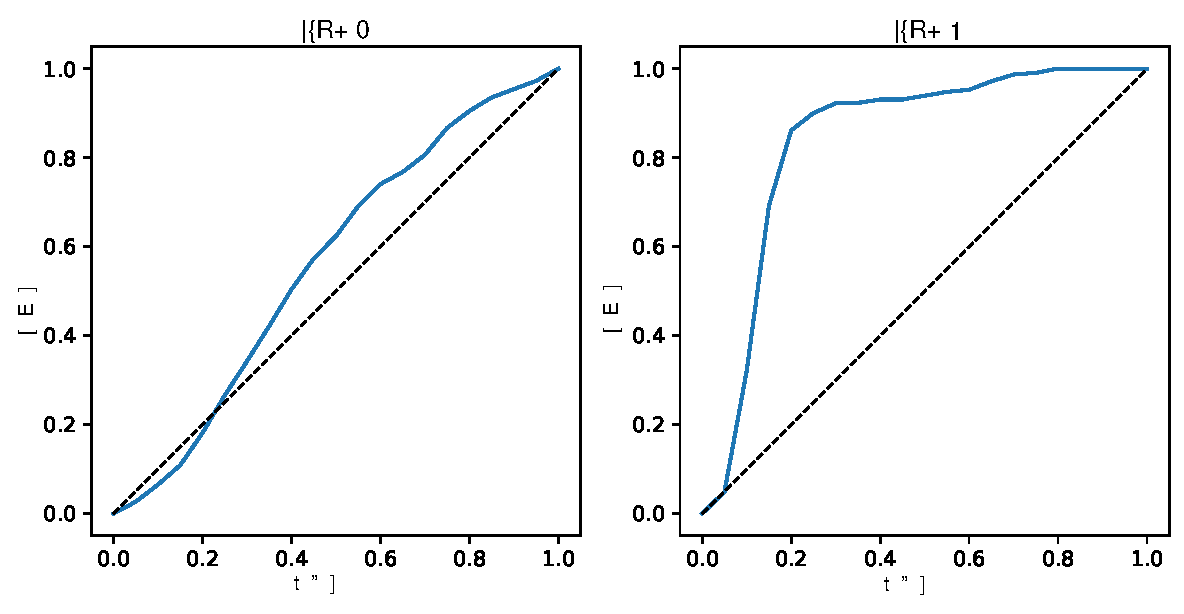
\includegraphics[width=1\linewidth]{Img/chapter8/invalidity}
$$\Downarrow \quad \textsf{经过蒙德里安一致性预测校正} \quad \Downarrow$$
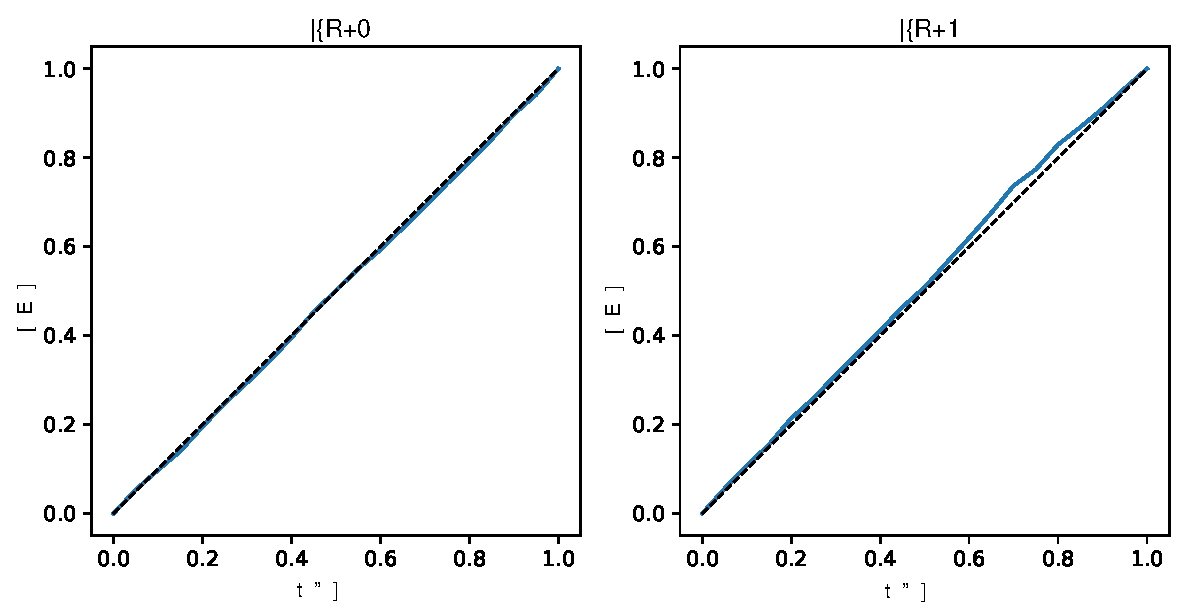
\includegraphics[width=1\linewidth]{Img/chapter8/validity}
\caption{MCP方法校正前后无人机集群真实数据集错误控制对比}
\label{fig:validity}
\end{figure}

\subsection{试验二:多元无人机集群行为分类研究}
针对复杂无人机集群行为分类问题, 在仿真数据上考虑生成多种无人机集群行为, 此问题是为多类别分类问题提供不确定量化。因此, 在无人机集群行为仿真数据集的研究中, 需要处理多类别分类任务。

基于第\ref{sec:dynamic}节所述的无人机集群动力学模型, 仿真三种具有代表性的无人机集群行为, 分别记为排列(Align)行为(标记为0), 聚集(Flock)行为(标记为1)和组队(Group)(标记为2)。 其他无人机集群的个体规模按照表\ref{tab:train_test}设置相同的参数。 同样的, 将仿真数据集按照$1:1:1$比例随机划分为真实训练集$Z_{proper}$, 校正集合$Z_{calibration}$和测试集$Z_{test}$。利用真实训练集$Z_{proper}$训练底层Boosting算法。

表\ref{tab:sys-simple-prediction}列出的是针对无人机集群行为仿真数据集, 蒙德里安一致性预测给出的置信预测结果。 例如, 对于第0号样例, 类别0,1,2对应计算得到的p-值分别是0.41, 0.33和0.26。 根据蒙德里安一致性预测理论其预测标签为0(此样例的蒙德里安一致性预测给出正确预测结果), 此时这种预测结果对应的置信度和可信度分别为0.67和0.41。 对于第1号样例, 类别0,1,2对应计算得到的p-值分别是0.34, 0.44和0.22。 根据蒙德里安一致性预测理论其预测标签为1(此样例的蒙德里安一致性预测给出错误预测结果), 此时这种预测结果对应的置信度和可信度分别为0.66和0.44。 对于第2号样例, 类别0,1,2对应计算得到的p-值分别是0.19, 0.34和0.47。 根据蒙德里安一致性预测理论其预测标签为2(此样例的蒙德里安一致性预测给出正确预测结果), 对应的置信度和可信度分别为0.66和0.47。

\begin{table}[]
\caption{无人机集群仿真数据集的置信预测结果示例表}
\label{tab:sys-simple-prediction}
\centering
\begin{tabular}{lrrrrrrr}
\toprule
\multicolumn{1}{c}{\begin{tabular}[c]{@{}c@{}}示例\\ 样本\end{tabular}} & \multicolumn{1}{c}{\begin{tabular}[c]{@{}c@{}}排列行为\\(标记为0)\end{tabular}} & \multicolumn{1}{c}{\begin{tabular}[c]{@{}c@{}}聚集行为\\(标记为1)\end{tabular}}  & \multicolumn{1}{c}{\begin{tabular}[c]{@{}c@{}}组队行为\\ (标记为2)\end{tabular}}  &  \multicolumn{1}{c}{\begin{tabular}[c]{@{}c@{}}真实\\ 标签\end{tabular}} &  \multicolumn{1}{c}{\begin{tabular}[c]{@{}c@{}}MCP\\ 预测标签\end{tabular}} &  置信度 &  可信度 \\
\midrule
0 &  0.41 &  0.33 &  0.26 &     0 &    0 &   0.67 &   0.41 \\
1 &  0.34 &  0.44 &  0.22 &     2 &    1 &   0.66 &   0.44 \\
2 &  0.19 &  0.34 &  0.47 &     2 &    2 &   0.66 &   0.47 \\
3 &  0.26 &  0.49 &  0.25 &     1 &    1 &   0.74 &   0.49 \\
$\ldots$ &  {} &  {} &  {} &     {} &     {} &  {} &     {} \\
12003 &  0.37 &  0.18 &  0.45 &     2 &    2 &   0.63 &   0.45 \\
12004 &  0.50 &  0.38 &  0.12 &     0 &    0 &   0.62 &   0.50 \\
12005 &  0.52 &  0.30 &  0.18 &     0 &    0 &   0.70 &   0.52 \\
12006 &  0.24 &  0.45 &  0.31 &     1 &    1 &   0.69 &   0.45 \\
12007 &  0.14 &  0.14 &  0.72 &     2 &    2 &   0.86 &   0.72 \\
\bottomrule
\end{tabular}
\end{table}
表\ref{tab:sys-set-prediction}给出的是利用蒙德里安一致性预测算法, 在指定显著性水平取值$\epsilon=0.15, 0.2, 0.4$下的集合预测结果。对于第0号样本, 类别0,1,2对应计算得到的p-值分别是0.41, 0.33和0.26。 根据MCP理论其在显著性水平$\epsilon = 0.15, 0.2, 0.4$ 下的集合预测结果分别是 $[0, 1, 2]$(预测正确), $[0, 1, 2]$(预测正确)和$[0]$(预测正确)。对于第1号样本, 类别0,1,2对应计算得到的p-值分别是0.34, 0.44和0.22。 根据MCP理论其在显著性水平$\epsilon = 0.15, 0.2, 0.4$ 下的集合预测结果分别是 $[0, 1, 2]$(预测正确), $[0, 1, 2]$(预测正确)和$[1]$(预测错误)。对于第2号样本, 类别0,1,2对应计算得到的p-值分别是0.19, 0.34和0.47。 根据MCP理论其在显著性水平$\epsilon = 0.15, 0.2, 0.4$ 下的集合预测结果分别是 $[0, 1, 2]$(预测正确), $[ 1, 2]$(预测正确)和$[2]$(预测正确)。
\begin{table}[]
\caption{无人机集群仿真数据集的集合预测结果示例表}
\label{tab:sys-set-prediction}
\centering
\begin{tabular}{lrrrlllr}
\toprule
\multicolumn{1}{c}{\begin{tabular}[c]{@{}c@{}}示例\\ 样本\end{tabular}} & \multicolumn{1}{c}{\begin{tabular}[c]{@{}c@{}}排列行为\\(标记为0)\end{tabular}} &  \multicolumn{1}{c}{\begin{tabular}[c]{@{}c@{}}聚集行为\\(标记为1)\end{tabular}}  &   \multicolumn{1}{c}{\begin{tabular}[c]{@{}c@{}}组队行为\\(标记为2)\end{tabular}} &       0.15 &        0.2 &  0.4 &  \multicolumn{1}{c}{\begin{tabular}[c]{@{}c@{}}真实\\标签\end{tabular}} \\
\midrule
0 &  0.41 &  0.33 &  0.26 &  [0, 1, 2] &  [0, 1, 2] &  [0] &     0 \\
1 &  0.34 &  0.44 &  0.22 &  [0, 1, 2] &  [0, 1, 2] &  [1] &     2 \\
2 &  0.19 &  0.34 &  0.47 &  [0, 1, 2] &     [1, 2] &  [2] &     2 \\
3 &  0.26 &  0.49 &  0.25 &  [0, 1, 2] &  [0, 1, 2] &  [1] &     1 \\
$\ldots$ &  {} &  {} &  {} &     {} &     {} &  {} &     {} \\
12003 &  0.37 &  0.18 &  0.45 &  [0, 1, 2] &     [0, 2] &  [2] &     2 \\
12004 &  0.50 &  0.38 &  0.12 &     [0, 1] &     [0, 1] &  [0] &     0 \\
12005 &  0.52 &  0.30 &  0.18 &  [0, 1, 2] &     [0, 1] &  [0] &     0 \\
12006 &  0.24 &  0.45 &  0.31 &  [0, 1, 2] &  [0, 1, 2] &  [1] &     1 \\
12007 &  0.14 &  0.14 &  0.72 &        [2] &        [2] &  [2] &     2 \\
\bottomrule
\end{tabular}
\end{table}

同样的, 也针对无人机集群仿真数据集检验经过蒙德里安一致性预测校正后各个类别的错误控制。结果不难发现, 如图\ref{fig:sys-validity}所示, 在采用蒙德里安一致性预测校正之前的机器学习算法对于每个类别的错误控制是失效的, 而经过蒙德里安一致性预测算法校正后每个类别的错误控制都能够和理论要求的错误控制保持一致。
\begin{figure}[]
\centering
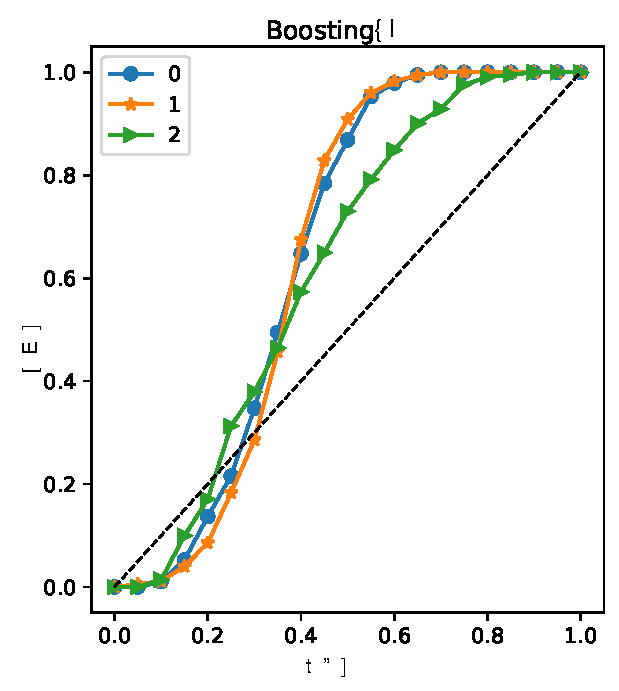
\includegraphics[width=.4\linewidth]{Img/chapter8/boost-invalidity}
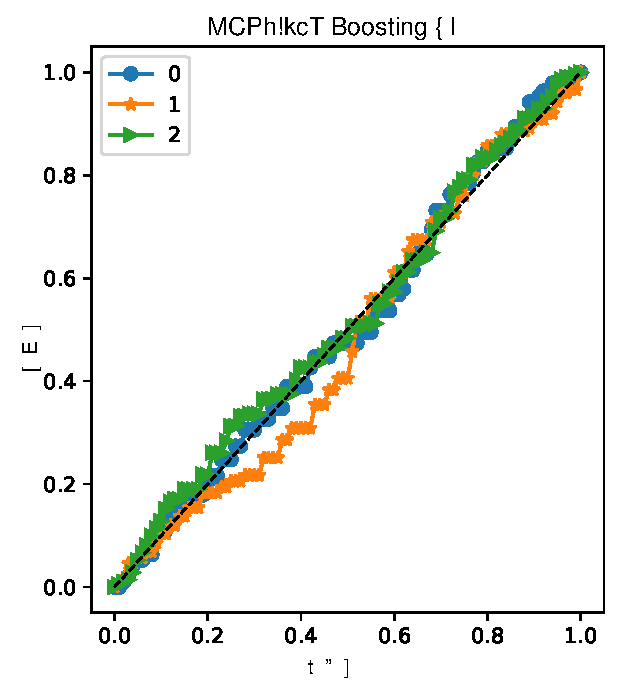
\includegraphics[width=.4\linewidth]{Img/chapter8/boosting-validity}
\caption{MCP方法校正前后无人机集群仿真数据集错误控制对比}
\label{fig:sys-validity}
\end{figure}

\section{本章小结}
\label{sec:discussion}
本章将Boosting算法作为底层机器学习算法, 利用一致性预测理论为无人机集群行为分类提供不确定量化。主要结论总结如下:
\begin{enumerate}
\item 针对二元无人机集群行为真实数据和多元无人机集群仿真数据, 提出采用一致性预测方案为机器学习分类算法输出结果提供无分布假设的不确定量化, 给出置信预测模式。试验数据表明, 一致性预测理论给出置信预测模式的有效性是自动满足的;
\item 针对二元无人机集群行为真实数据和多元无人机集群仿真数据, 提出采用一致性预测方案给出集合预测模式。试验数据表明, 集合预测能够实现在任意显著性水平下有保证的多类别预测结果;
\item 检验经过一致性预测校正前后各个类别的错误控制。试验数据表明, 未经一致性预测理论校正的常规机器学习算法无法达到有效错误控制; 经过一致性预测方法校正后, 每个类别的错误控制都得到有效控制, 使得理论误差和实际误差保持一致。
\end{enumerate}
